\chapter{Umsetzung des Prototypen}

Die Umsetzung des Prototypen entspricht dem Hauptteil dieser Arbeit. Ziel ist es einen Augmented-Reality-Anwendung zu entwickeln, die die Montage von Rauchmeldern unterstützt und die Regeln bei der Positionierung in einer augmentierten Umgebung visualisiert. Dabei sollen Smartphones und Tablets sowohl als Eingabe- als auch als Ausgabegeräte genutzt werden. Im Folgenden werden die einzelnen Schritte der Umsetzung erläutert, einschließlich der Beschreibung der Anforderungen, Konzeption und Implementierung.

\section{Anforderungen}\label{sec:requirements}

Um eine zielgerichtete Entwicklung des Prototyps zu gewährleisten, müssen zunächst die Anforderungen definiert werden. Sie dienen als Grundlage für die weitere Konzeption und Implementierung der Anwendung. Dabei wurden verschiedene Einflussfaktoren berücksichtigt, die die Anforderungen an das System maßgeblich bestimmen.

\subsection{Benutzerinteraktion}

Die Gestaltung der Benutzerinteraktion in Augmented-Reality-Anwendungen muss sorgfältig geplant werden, um eine intuitive und benutzerfreundliche Bedienung zu gewährleisten. Die Interaktionen sollten einfach und schnell durchführbar sein, um den Benutzer nicht zu überfordern. Der Benutzer sollte sofort erkennen können, wie er mit der Anwendung interagieren kann. 

Denkbare Interaktionsmöglichkeiten umfassen unter anderem Handgesten vor der Kamera, Sprachbefehle oder Touch-Gesten. Allerdings sind die verfügbaren Interaktionsformen durch die Nutzung von Smartphones und Tablets eingeschränkt. Dies liegt vor allem daran, dass das Gerät während der Anwendung in der Hand gehalten werden muss. Besonders bei Tablets kann es notwendig sein, beide Hände zur Stabilisierung des Geräts einzusetzen.

Unter der Annahme, dass das Tablet, wie in Abbildung \ref{fig:ipad} dargestellt, mit beiden Händen gehalten wird, beschränken sich die möglichen Interaktionen auf die Daumen des Benutzers sowie auf die Positionierung und Ausrichtung des Geräts. Daher sollten die Interaktionsmechanismen der AR-Anwendung möglichst einfach und minimalistisch gestaltet sein, um eine komfortable Bedienung zu ermöglichen, ohne dass das Risiko besteht, das Gerät versehentlich fallen zu lassen.

[Bild: iPad]

\subsection{Genauigkeit}

Die Visualisierung von Montageregeln für Rauchmelder erfordert eine hohe Genauigkeit bei der Tiefenmessung und dem Tracking der Umgebung. Wie einleitend beschrieben, können fehlerhafte Montagen schwerwiegende Folgen haben. Daher ist es essenziell sicherzustellen, dass die Dimensionen des virtuellen Koordinatensystems, in dem die Rauchmelder platziert werden, exakt mit der realen Welt übereinstimmen. Nur so können Abstände korrekt gemessen und die Montageregeln präzise visualisiert werden.

\subsection{Echtzeit-Darstellung}

Die Echtzeitleistung der Darstellung der Augmented-Reality-Szene spielt eine entscheidende Rolle in AR-Anwendungen. Es ist wichtig, Latenzen und Drift-Effekte zu minimieren, um sicherzustellen, dass virtuelle Objekte exakt und synchron mit der realen Welt dargestellt werden. Eine effiziente Verarbeitung der Sensordaten sowie die präzise Positionierung und Darstellung der virtuellen Objekte sind daher essenziell. Gleichzeitig dürfen diese Prozesse nicht miteinander in Konflikt geraten oder sich gegenseitig blockieren. Auch Benutzerinteraktionen sollten ohne Verzögerungen erfolgen, um das Erlebnis nicht negativ zu beeinflussen.

\subsection{User-Feedback}

Das User-Feedback ist ein wichtiger Bestandteil von Augmented-Reality-Anwendungen, da es dem Benutzer hilft, den aktuellen Zustand des Systems zu verstehen. AR-Systeme können je nach Tracking-Status unerwartete oder fehlerhafte Darstellungen liefern. Daher ist es essenziell, den Nutzer kontinuierlich über den Status der Anwendung zu informieren.

Zudem sollte das System auf mögliche Fehlbedienungen hinweisen und dem Benutzer gezielte Hilfestellungen bieten, um Korrekturen vorzunehmen. Dies kann durch visuelle Indikatoren, Textnachrichten oder andere Formen der Rückmeldung, wie akustische oder haptische Signale, erfolgen. Ein gut durchdachtes Feedback-System verbessert nicht nur die Benutzererfahrung, sondern trägt auch zur intuitiven Bedienbarkeit der Anwendung bei.

\subsection{Verzicht auf manuelle Kalibrierung und Initialisierung}

Falls die Anwendung in einem professionellen Umfeld eingesetzt werden soll, ist es wichtig, dass die Anwendung eine möglichst geringe Einstiegshürde aufweist. Dies bedeutet, dass die Anwendung ohne manuelle Kalibrierung oder Initialisierung starten sollte. Der Benutzer sollte die Anwendung starten und sofort mit der Interaktion beginnen können. Dies ist besonders wichtig, wenn die Anwendung in Geschäftsprozessen eingesetzt wird, in denen Zeit ein kritischer Faktor ist.

\section{Konzeption}

Das Konzept des Prototypen wurde iterativ entwickelt und nicht in einem einzigen Schritt abgeschlossen. Dabei wurden die Lösungsansätze schrittweise umgesetzt und kontinuierlich optimiert, um die Anforderungen bestmöglich zu erfüllen. Zu Beginn wurde eine grundlegende Skizze des Prototyps erstellt (siehe Abbildung \ref{fig:Concept}), die die zentralen Funktionen und Interaktionen veranschaulichte. Diese diente als Ausgangspunkt für die weitere Entwicklung und half dabei, die wesentlichen Komponenten des Systems frühzeitig zu definieren.

Die Hauptkomponenten des ersten Konzepts umfassten die folgenden Funktionen:

\begin{itemize}
    \item \textbf{Anzeige von Flächen:} Die Anwendung soll in der Lage sein, Flächen in der Umgebung zu erkennen und anzuzeigen.
    \item \textbf{Darstellung der Montageregeln:} Die Montageregeln sollen direkt an der Decke in Form von Farbflächen dargestellt werden.
    \item \textbf{Automatische Platzierung eines virtuellen Rauchmelders:} Der Prototyp soll, basierend auf den erkannten Flächen und den Montageregeln, in der Lage sein, einen virtuellen Rauchmelder automatisch an die optimale Position zu platzieren.
    \item \textbf{Darstellung des Rauchmelders:} Virtuelle Rauchmelder sollen in der augmentierten Umgebung dargestellt werden, um dem Benutzer eine genaue Vorstellung von deren Position zu geben.
    \item \textbf{Distanzindikatoren:} Um sicherzustellen, dass die Rauchmelder korrekt montiert werden, sollen Distanzindikatoren visualisiert werden, die dem Benutzer die Abstände zu den umgebenden Wänden anzeigen.
    \item \textbf{Informationsanzeige:} Die Anwendung soll dem Benutzer zusätzliche Informationen anzeigen, wie z.B. den Status der Platzierung und Hinweise zur optimalen Positionierung.
\end{itemize}

Auch wenn dieses erste Konzept eine gute Grundlage für die weitere Entwicklung darstellte, mussten im Laufe der Implementierung einige Anpassungen aufgrund neuer Erkenntnisse vorgenommen werden. Eine Erkenntnis war, dass die automatische Platzierung des Rauchmelders die Erfahrung und Intuition des Monteurs vernachlässigte. Aus diesem Grund wurde eine sogenannte \emph{Focus-Entity} eingeführt, die dem Benutzer die Möglichkeit gibt, den Rauchmelder manuell zu platzieren. Diese Entity stellt einen abstrakten, virtuellen Rauchmelder im Raum dar, der stets im Fokus des Benutzers, also in der Mitte des Bildschirms, bleibt. Der Benutzer kann den Rauchmelder durch die Bewegung und Ausrichtung des Gerätes positionieren. Dadurch wird eine intuitive Benutzerinteraktion gewährleistet und die Arbeit des Monteurs unterstützt anstatt sie zu ersetzen.

Mit der Einführung der Focus-Entity wurde eine geeignete Interaktionsmethode erforderlich. Dabei wurden verschiedene Interaktionsmöglichkeiten wie Handgesten, Sprachbefehle und physische Tasten in Betracht gezogen. Letztlich fiel die Wahl auf Touch-Gesten, da diese bereits in vielen Anwendungen etabliert sind und dem Benutzer eine vertraute Bedienweise bieten. Zusätzlich dazu liefern die Icons der Schaltflächen des User-Interfaces bereits visuelle Rückmeldungen, die dem Benutzer zeigen, wie er mit der Anwendung interagieren kann ohne ihn zunächst mit der Bedienung vertraut machen zu müssen. Der Benutzer kann somit den Rauchmelder an der aktuellen Position der Focus-Entity platzieren, sofern es sich um eine gültige Position handelt.

Die Anzahl der notwendigen Interaktionen wurde bewusst auf ein Minimum reduziert, um eine möglichst effiziente Bedienung zu gewährleisten. Der Monteur soll nur dann aktiv mit dem Bildschirm interagieren müssen, wenn es unbedingt erforderlich ist. Daher wurde sorgfältig abgewogen, wieviele Schaltflächen und UI-Elemente für die einwandfreie Nutzung der Anwendung erforderlich sind. In diesem Zusammenhang wurden drei wesentliche Interaktionen als notwendig erachtet:

\begin{itemize}
    \item Platzieren des Rauchmelders
    \item Löschen des Rauchmelders
    \item Bildschirmfoto der Szene machen
\end{itemize}

Die Interaktionen wurden als Schaltflächen am unteren Rand des Bildschirms platziert. Die Schaltflächen sind so angeordnet, dass sie mit den Daumen erreicht werden können, ohne in irgendeiner Art und Weise umgreifen zu müssen. 

Ein weiteres zentrales Element der Benutzeroberfläche ist die Informationsanzeige, die dem Benutzer jederzeit den aktuellen Status der Platzierung vermittelt. Um die Sicht auf die augmentierte Umgebung nicht zu beeinträchtigen, wurde sie am oberen rechten Rand des Bildschirms platziert. Statusänderungen werden durch Animationen hervorgehoben, um die Aufmerksamkeit des Benutzers gezielt darauf zu lenken. Ein zusätzliches Info-Icon dient als Ankerpunkt für das Textfeld und erleichtert die Einordnung der gezeigten Informationen.

[Evtl. Bildersequenz der Animation]

Um eine gültige Position für den Rauchmelder visuell zu verdeutlichen, wurden zwei Indikatoren implementiert. Zum einen ändert sich die Farbe der Focus-Entity sowie des Info-Icons, sobald sich der Rauchmelder an einer gültigen Position befindet. Zum anderen wird ein zusätzlicher Ring um die Focus-Entity angezeigt, der einen Abstand von 0,6 Metern gemäß den Montageregeln (gemäß Regeln 2 und 3, siehe \ref{cha:Problemstellung}) visualisiert. Dadurch erhält der Benutzer direktes Feedback zur Einhaltung der Mindestanforderungen und kann die Platzierung entsprechend anpassen.

[Bild: Indikator auf gültiger Position]

\section{Auswahl der Technologien}

Für die Umsetzung des Prototypen wurden verschiedene Technologien und Frameworks in Betracht gezogen. Dabei wurden die Anforderungen an die Anwendung und die verfügbaren Ressourcen berücksichtigt. Da die Anwendung primär für mobile Endgeräte wie Smartphones und Tablets konzipiert wurde, lag der Fokus auf plattformgerechten Technologien mit leistungsfähiger AR-Unterstützung.

Ein zentrales Kriterium bei der Wahl der Technologien war die Beschaffenheit der Deckenoberflächen, da diese in der Regel glatt sind und somit nur wenige markante Merkmale für das visuelle Tracking bieten. Diese begrenzte Anzahl an Feature-Punkten kann dazu führen, dass das Tracking instabil wird und virtuelle Objekte nicht präzise in der Umgebung verankert werden können. Erste Tests mit dem ARCore-Framework von Google zeigten, dass dessen Tracking-Mechanismus (vSLAM) auf glatten Oberflächen an seine Grenzen stößt. Abbildung \ref{fig:ARCore} zeigt eine Demo-Anwendung von Google, die die Anzahl der erkannten Feature-Punkte anzeigt. Dabei wird deutlich, dass ARCore auf einer glatten Decke nur wenige Referenzpunkte identifizieren kann, was zu einer eingeschränkten Tracking-Stabilität führt, wenn man davon ausgeht dass die Kamera primär auf die Decke gerichtet ist.

[Bild: ARCore Demo]

Aufgrund dieser Limitation erwiesen sich Frameworks, die LiDAR-gestütztes Tracking unterstützen, als eine vielversprechende Alternative. Wie bereits in Kapitel \ref{LiDAR} beschrieben, ermöglicht LiDAR eine präzise Tiefenerfassung und eine zuverlässige Flächenerkennung – unabhängig von der Oberflächenstruktur. Darüber hinaus reduziert LiDAR die Initialisierungszeit, da die Tiefeninformationen fast augenblicklich verfügbar sind. Ein weiterer Vorteil ist, dass LiDAR-Sensoren unabhängig vom Umgebungslicht funktionieren, was besonders für professionelle Anwendungen von Bedeutung ist, da die Lichtverhältnisse in Gebäuden nicht immer optimal sind.

Allerdings sind aktuell nur wenige mobile Geräte mit einem LiDAR-Sensor ausgestattet. Besonders im Android-Segment gibt es derzeit keine Geräte mit einem rückseitig integrierten LiDAR-Sensor. Daher fiel die Entscheidung auf die Entwicklung eines iOS-basierten Prototyps unter Verwendung eines iPad Pro der dritten Generation. Dieses Gerät bietet sowohl die benötigte Rechenleistung als auch einen leistungsfähigen LiDAR-Sensor, der sich ideal für die Umsetzung eignet. Die Wahl von iOS als Plattform machte den Einsatz der Programmiersprache Swift erforderlich, da diese speziell für die Entwicklung von Anwendungen auf Apple-Geräten optimiert ist. Zudem wurde ein MacBook Air als Entwicklungsumgebung verwendet, da ein macOS-basiertes System notwendig ist, um die Anwendung auf das iPad zu übertragen und zu testen.

Für die Augmented-Reality-Funktionalitäten wurde das ARKit-Framework von Apple eingesetzt, da es speziell für iOS-Geräte entwickelt wurde und eine Vielzahl von Funktionen für AR-Anwendungen bietet. Dazu gehören unter anderem das Tracking der Umgebung, die Erkennung von Flächen, die präzise Platzierung virtueller Objekte sowie die Objekterkennung und -klassifizierung. Besonders vorteilhaft ist die enge Integration von ARKit mit der LiDAR-Technologie, die eine hohe Genauigkeit und Stabilität bei der Platzierung von virtuellen Objekten ermöglicht. Ein Nachteil von ARKit besteht jedoch darin, dass es sich um eine weitgehend geschlossene Lösung handelt, deren interne Funktionsweise nicht vollständig dokumentiert ist. Durch Analyse der Dokumentation und von Logging-Informationen lässt sich jedoch darauf schließen, dass ARKit ein SLAM-Verfahren unter Verwendung der Fusion von Kameradaten, LiDAR-Daten und Sensordaten der IMU verwendet.

Zusätzlich wurde ARKit mit dem RealityKit-Framework kombiniert, das speziell für die Darstellung und Interaktion mit 3D-Objekten in einer augmentierten Umgebung entwickelt wurde. RealityKit bietet eine leistungsfähige Render-Engine, die unter anderem physikalisch basierte Beleuchtung, Animationen und Echtzeitinteraktionen mit 3D-Objekten unterstützt. Durch die enge Verzahnung mit ARKit wird eine hohe Performance bei der Visualisierung von augmentierten Inhalten erreicht, was die Entwicklung des Prototyps erheblich erleichterte.

Durch diese Technologieauswahl konnte eine stabile, performante und präzise AR-Anwendung realisiert werden, die insbesondere auf die Herausforderungen glatter Oberflächen und anspruchsvoller Tracking-Bedingungen optimiert ist.

\section{Implementierung des Prototypen}

Die Implementierung des Prototypen erfolgte in mehreren Schritten, die sich an den Anforderungen und dem Konzept orientierten. Dabei wurden die zentralen Funktionen und Komponenten schrittweise entwickelt und getestet, um eine reibungslose Funktionalität und eine intuitive Benutzererfahrung zu gewährleisten. Im Folgenden werden die wichtigsten Aspekte der Implementierung beschrieben.

\subsection{Softwarearchitektur}

Die Softwarearchitektur des Prototyps wurde so konzipiert, dass sie flexibel, modular und erweiterbar ist, um zukünftige Anforderungen und Anpassungen problemlos zu ermöglichen. Dabei kommt das \emph{Model-View-ViewModel} (MVVM)-Pattern zum Einsatz, das eine klare Trennung zwischen Datenstrukturen, Geschäftslogik und Benutzeroberfläche gewährleistet. Abbildung \ref{fig:Architecture} stellt eine Übersicht über die Architektur des Prototypen dar.

\begin{figure}[ht]
    \centering
    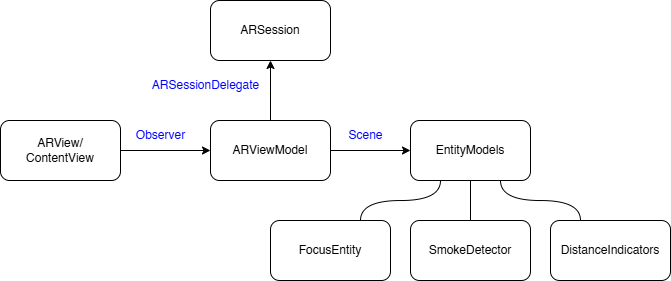
\includegraphics[width=0.8\textwidth]{Architecture}
    \caption{Softwarearchitektur des Prototypen}
    \label{fig:Architecture}
\end{figure}

Die \emph{View}-Schicht ist für die Darstellung der Augmented-Reality-Szene und der UI-Elemente zuständig. Sie beobachtet das \texttt{ARViewModel} und aktualisiert die Anzeige basierend auf den empfangenen Daten. Das \texttt{ARViewModel} bildet die zentrale Steuerungseinheit der Anwendung. Es verwaltet die Kommunikation mit der \texttt{ARSession}, empfängt Tracking-Daten und verarbeitet Änderungen in der AR-Umgebung. Darüber hinaus aktualisiert es die Szene durch das Verwalten und Steuern der enthaltenen Augmented-Reality-Objekte.

Die AR-Objekte entsprechen Subklassen der \texttt{EntityModel}-Klasse. Für die Implementierung des Prototypen wurden die folgenden Entitäten definiert:

\begin{itemize}
    \item \texttt{FocusEntity}: dient als visuelle Orientierungshilfe für den Nutzer und markiert potenzielle Platzierungsorte
    \item \texttt{SmokeDetector}: repräsentiert den virtuellen Rauchmelder innerhalb der AR-Umgebung
    \item \texttt{DistanceIndicators}: zeigen Abstände zu den umgebenden Flächen an, um die korrekte Montage sicherzustellen
\end{itemize}

Die Kommunikation zwischen diesen Komponenten erfolgt mithilfe des \texttt{Observer}-Patterns. Die View beobachtet dabei das \texttt{ViewModel} und reagiert auf Änderungen in der Szene. Dank des in Swift integrierten Observation-Frameworks lässt sich dieses Muster einfach umsetzen, ohne zusätzlichen Boilerplate-Code zu erzeugen. Die Annotation \texttt{@Observable} ermöglicht es, dass Änderungen an einer Klasse automatisch an ihre Beobachter weitergeleitet werden \cite{appledevdoc}:

\begin{lstlisting}[language=Swift]
@Observable
class ARViewModel {
    private(set) var scene: [Entity & HasAnchor] = []
    @ObservationIgnored private var isProcessing: Bool = false
    // ...
}
\end{lstlisting}

Variablen, die nicht beobachtet werden sollen, können mit \texttt{@ObservationIgnored} markiert werden, wodurch unnötige Updates vermieden und die Performance optimiert wird. \cite{appledevdoc}

Das \texttt{ViewModel} erhält kontinuierlich Tracking-Daten von der \texttt{ARSession}, indem es das \texttt{ARSessionDelegate}-Protokoll implementiert. Dieses stellt verschiedene Callback-Methoden bereit, mit denen auf Änderungen in der Umgebung reagiert werden kann. Die \texttt{ARSession} erfasst Sensordaten und liefert Informationen zu Kamerapositionen, erkannten Flächen sowie identifizierter Objekte. Das \texttt{ViewModel} verarbeitet diese Daten und aktualisiert daraufhin die \texttt{EntityModels}, um die Darstellung in der AR-Szene entsprechend anzupassen.

Durch diese Architektur wird eine klare Trennung der Verantwortlichkeiten erreicht, wodurch die Anwendung strukturiert, effizient und leicht erweiterbar bleibt. Neue Funktionen oder zusätzliche Entitäten können nahtlos integriert werden, ohne die bestehende Codebasis grundlegend verändern zu müssen.

\subsection{View}

Die Benutzeroberfläche des Prototyps wurde mit dem SwiftUI-Framework von Apple entwickelt. SwiftUI verwendet eine deklarative Syntax, um Benutzeroberflächen zu erstellen und zu verwalten. Dabei werden einzelne \texttt{View}-Komponenten als grundlegende Bausteine der Benutzeroberfläche verwendet, die durch Modifikatoren und Container zu komplexen Layouts zusammengesetzt werden können. \cite{appledevdoc}

Der komponentenbasierte Aufbau der Benutzeroberfläche lässt sich ideal als Baumstruktur visualisieren:

\begin{figure}[h]
    \centering
    \begin{minipage}{0.45\textwidth}
        \centering
        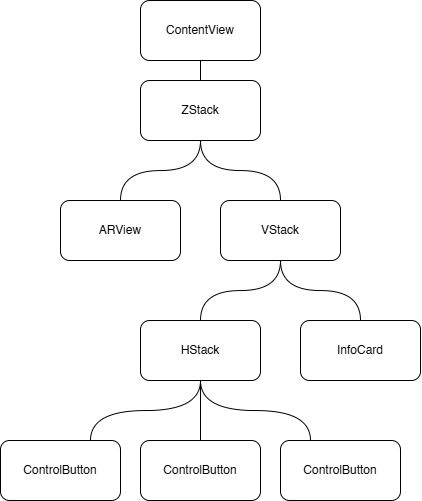
\includegraphics[width=\textwidth]{UI}
    \end{minipage}
    \hfill
    \begin{minipage}{0.45\textwidth}
        \centering
        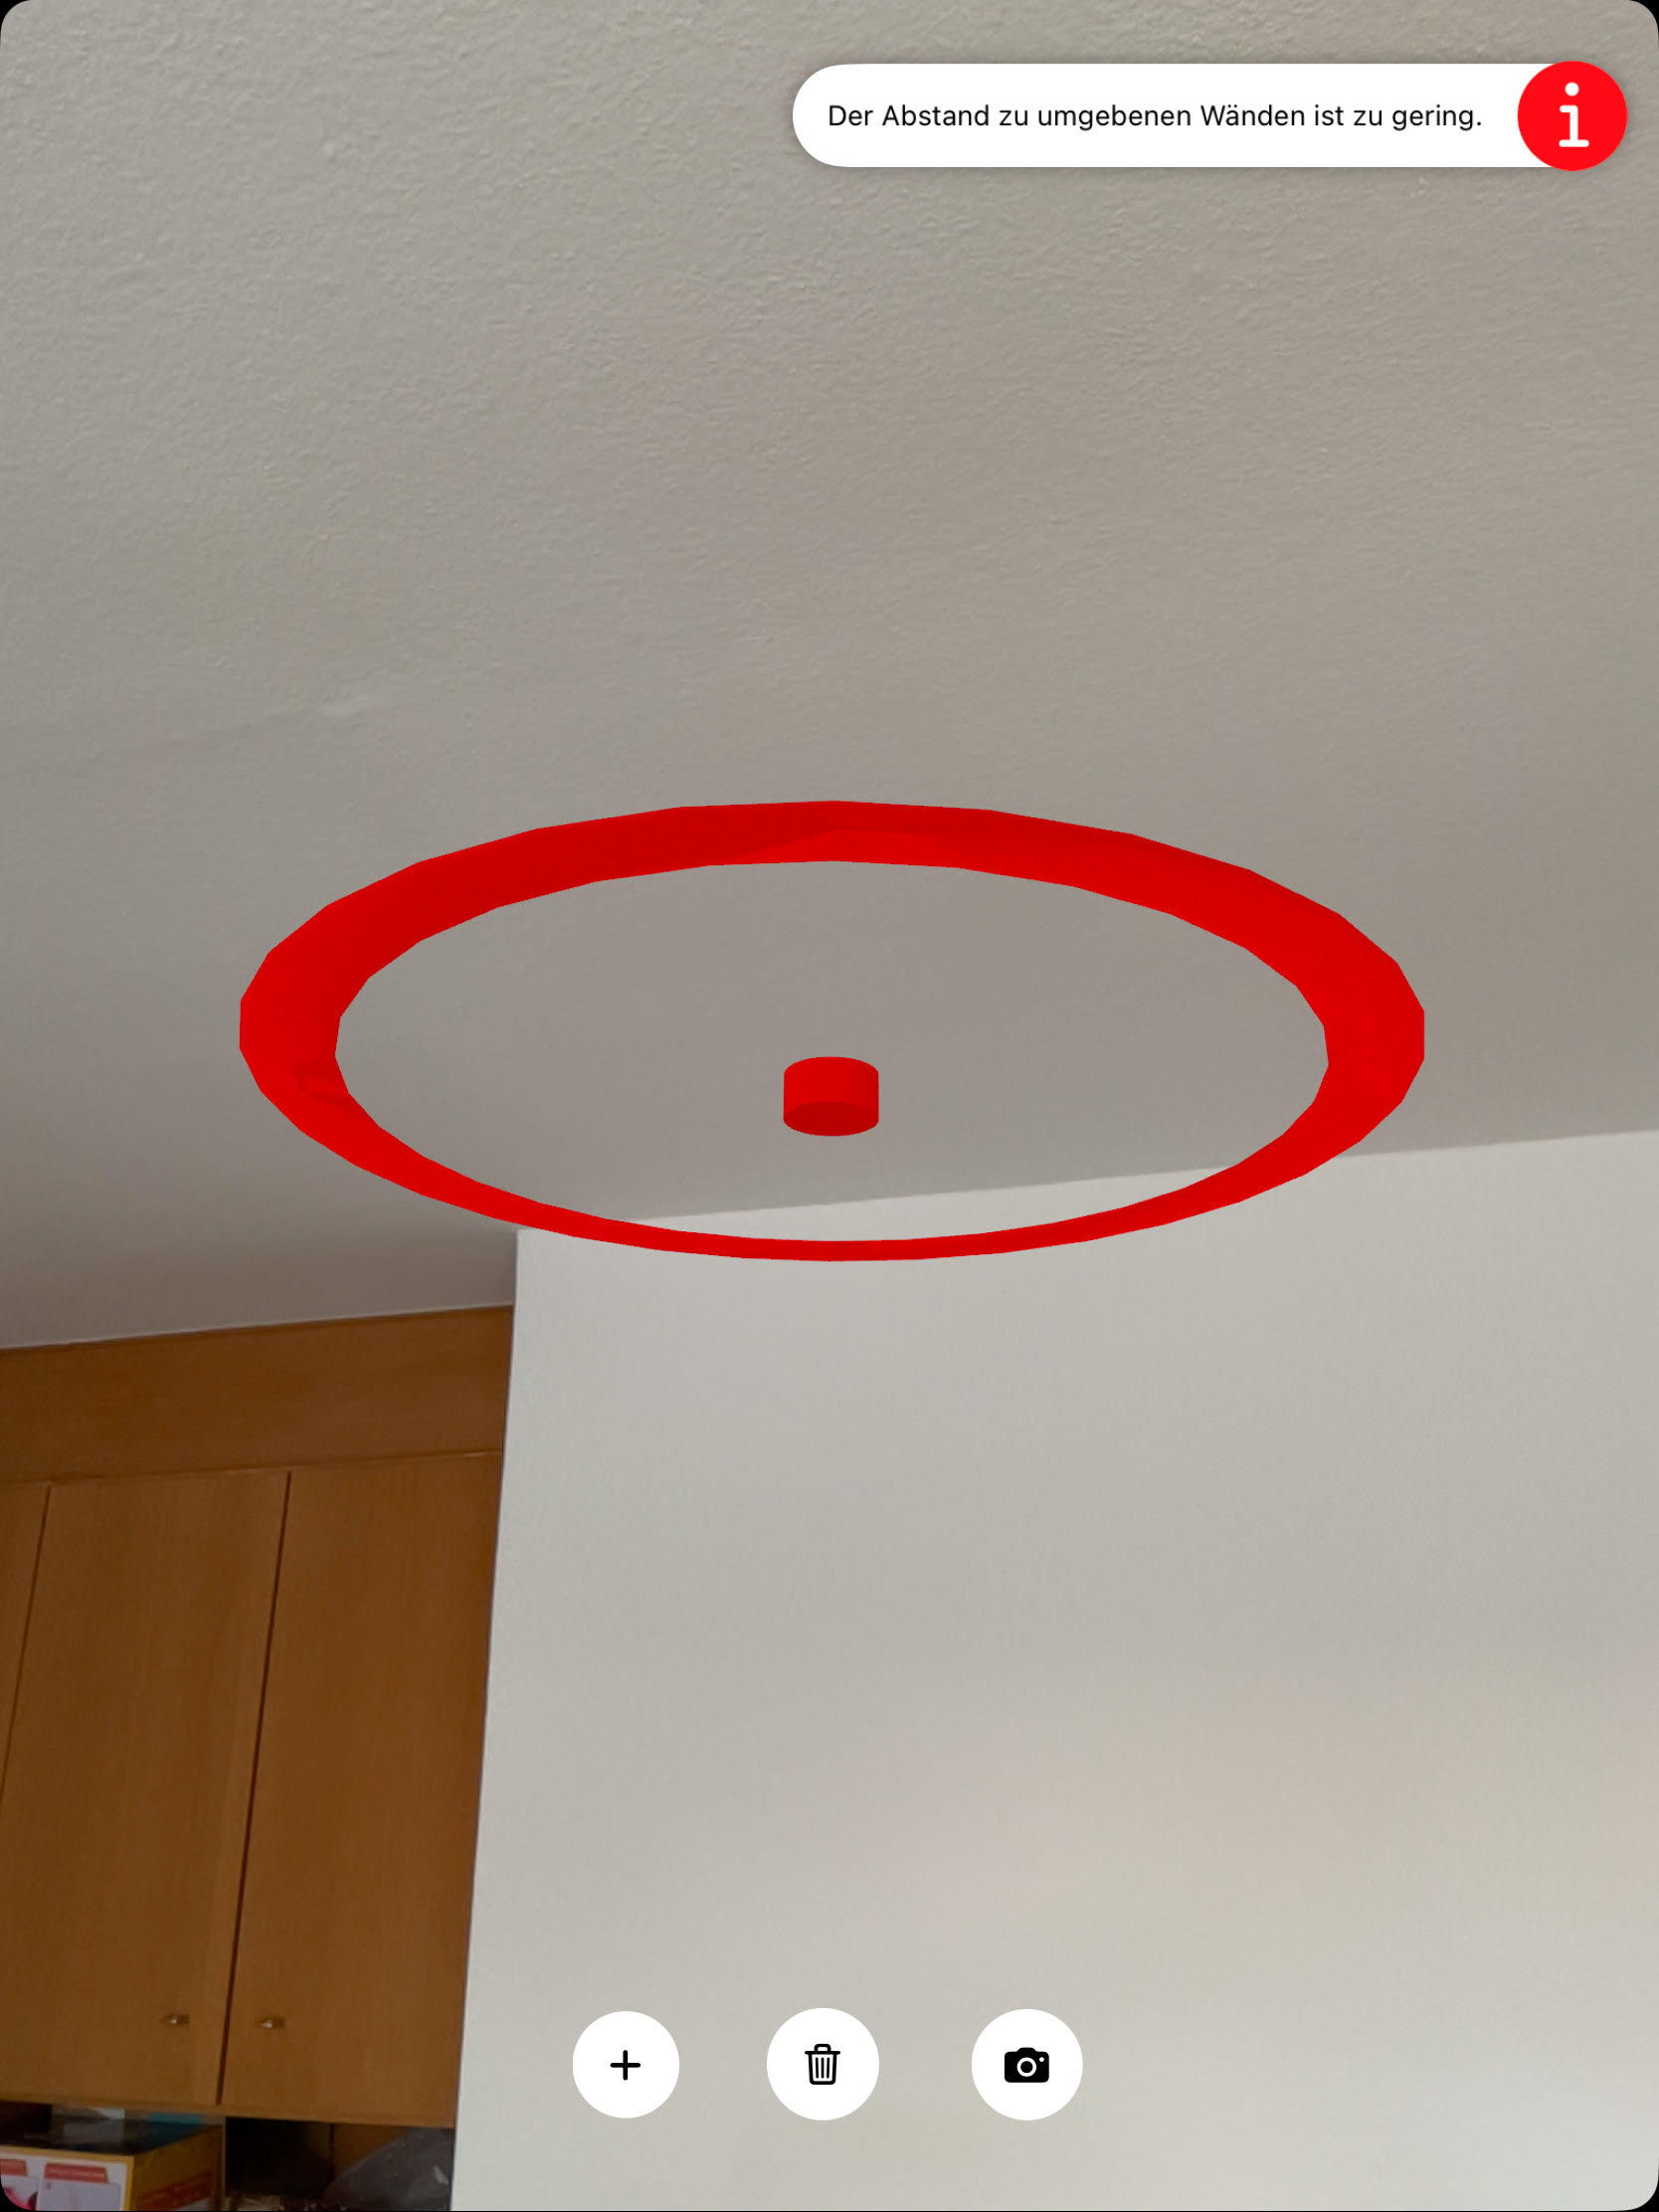
\includegraphics[width=\textwidth]{AppUI}
    \end{minipage}
    \caption{SwiftUI-Benutzeroberfläche: Baumstruktur (links) und App-Ansicht (rechts)}
    \label{fig:AppUI}
\end{figure}

Dieser modulare Aufbau ermöglicht eine strukturierte und flexible Implementierung der Benutzeroberfläche, wobei jede Komponente eigenständig und wiederverwendbar ist. Ein Beispiel hierfür ist der \texttt{ControlButton}, der mehrfach mit verschiedenen Symbolen und zugehörigen Callback-Funktionen eingesetzt wird.

\begin{lstlisting}[language=Swift]
struct ControlButton: View {
    var iconName: String
    var action: () -> Void
        
    var body: some View {
        // Implementatierung der Button-Komponente
    }
}
\end{lstlisting}

SwiftUI stellt eine Vielzahl vordefinierter Komponenten bereit, die speziell für die Entwicklung von iOS-Anwendungen optimiert sind. So kommt beispielsweise die \texttt{ZStack}-Komponente zum Einsatz, um die Buttons und die InfoCard über der ARView zu platzieren.

Zur Steuerung der Darstellung und des Verhaltens der Komponenten wurden Modifikatoren verwendet. Ein Beispiel hierfür ist die Verwendung von Übergängen und Animationen, um die Zustandsänderungen der \texttt{InfoCard} visuell darzustellen:

\begin{lstlisting}[language=Swift]
InfoText(infoText: infoText)
    .transition(.move(edge: .trailing))
    .animation(.easeInOut(duration: 0.5), value: infoText)
    .opacity(infoText.isEmpty ? 0 : 1)
    .animation(.easeInOut(duration: 0.4), value: infoText)
\end{lstlisting}

Der \texttt{transition}-Modifikator stellt eine Bewegung der Komponent von der rechten Bildschirmkante dar. Diese Bewegung wird durch den \texttt{animation}-Modifikator animiert. Um den Übergangseffekt zu verstärken, wird zusätzlich der \texttt{opacity}-Modifikator verwendet, um die Transparenz der Komponente während des Übergangs zu steuern.

Die ARView bildet das Herzstück der Augmented-Reality-Darstellung und ist Teil des RealityKit-Frameworks. Sie ermöglicht das Rendering von 3D-Objekten in einer erweiterten Umgebung. Um die ARView in die SwiftUI-View zu integrieren, muss sie als \texttt{UIViewRepresentable}-Komponente eingebunden werden. Dies erlaubt es, die ARView als Subview der SwiftUI-View zu verwenden, wo sie mithilfe von Modifikatoren positioniert und skaliert wird.

\subsection{Konfiguration und Nutzung der ARSession}

Die \texttt{ARSession} ist die zentrale Komponente des ARKit-Frameworks und bildet die Grundlage für die Entwicklung von Augmented-Reality-Anwendungen auf iOS-Geräten. Sie verwaltet das Tracking der Umgebung, die Verarbeitung von Sensordaten und die Bereitstellung von Ankerpunkten zur Platzierung virtueller Objekte. Für den Prototypen wurde die Session mit der folgenden Konfiguration initialisiert:

\begin{lstlisting}[language=Swift]
let config = ARWorldTrackingConfiguration()
config.planeDetection = [.horizontal, .vertical]
config.sceneReconstruction = .meshWithClassification
config.frameSemantics.insert(.sceneDepth)
\end{lstlisting}

Diese Konfiguration aktiviert zunächst die Erkennung horizontaler und vertikaler Flächen. Die \texttt{ARSession} erkennt diese \textit{Planes} mithilfe der Kameradaten und der Tiefeninformationen des LiDAR-Sensors. Die erkannten Flächen werden kontinuierlich optimiert und erweitert. Sie werden als \texttt{ARPlaneAnchor}-Objekte bereitgestellt, die Informationen zu Position, Ausrichtung und Größe der Fläche enthalten. Über das RealityKit-Framework können diese Ankerpunkte genutzt werden, um virtuelle Objekte stabil auf den erkannten Flächen zu platzieren.

Ein weiterer wesentlicher Bestandteil der Konfiguration ist die Aktivierung der Szenenrekonstruktion durch \texttt{.meshWithClassification}. Dabei wird die Umgebung auf Basis der LiDAR-Daten als detailliertes Mesh rekonstruiert. Diese Methode ermöglicht nicht nur eine präzisere Platzierung virtueller Objekte, sondern auch eine exakte Erfassung von Abständen und Größenverhältnissen. Zudem bietet ARKit eine semantische Klassifikation des Meshes, die es erlaubt, verschiedene Oberflächentypen zu unterscheiden. Dazu verwendet ARKit, die im Kapitel \ref{sec:SceneUnderstanding} beschriebene, semantische Segmentierung. Die Klassifizierung erfolgt nach den folgenden Kategorien:

\begin{lstlisting}[language=Swift]
    enum ARMeshClassification: Int {
        case ceiling
        case door
        case floor
        case none
        case seat
        case table  
        case wall
        case window
    }
\end{lstlisting}

Die Klassifizierung bezieht sich nicht nur auf ganze Meshes, sondern auch auf deren einzelne Faces. Dadurch kann die Anwendung gezielt zwischen verschiedenen Oberflächentypen unterscheiden, was insbesondere für die Darstellung der Montageregeln essenziell ist. Da diese Vorgaben spezifische Abstände zu Elementen wie Wänden, Fenstern oder Türen erfordern, ermöglicht diese Segmentierung eine exakte Bestimmung der Platzierung des Rauchmelders.

Das \texttt{ARModelView} fungiert als Delegierter (\emph{Delegate}) der \texttt{ARSession} und kann daher in Echtzeit auf die verarbeiteten Daten zugreifen, die in Form von \texttt{ARFrame}-Objekten bereitgestellt werden. Diese enthalten:

\begin{itemize}
    \item Informationen über das generierte Mesh und dessen Klassifikation,
    \item erkannte Flächen und ihre Positionen,
    \item zusätzliche Tiefendaten durch die aktivierte Frame-Semantik \texttt{.sceneDepth}.
\end{itemize}

\begin{tcolorbox}[colback=THAi-Blue!20!white, colframe=THAi-Blue]
    Ein Delegate ist ein Entwurfsmuster, bei dem ein Objekt die Verarbeitung bestimmter Ereignisse an ein konfigurierbares Delegate-Objekt auslagert. Dadurch kann z. B. eine Klasse auf Ereignisse reagieren, ohne sie selbst implementieren zu müssen. \cite{appledevdoc}
\end{tcolorbox}  

Diese Informationen nutzt das \texttt{ARModelView}, um die Entitäten in der Szene dynamisch anzupassen. Insbesondere die Klassifikationsdaten ermöglichen es, objektspezifische Platzierungsbedingungen zu berücksichtigen – etwa notwendige Mindestabstände zu Türen oder Fenstern. Die zusätzlichen Tiefeninformationen aus der \texttt{sceneDepth}-Semantik tragen ebenfalls zur verbesserten Positionierung virtueller Objekte bei, indem sie genauere Abstandsmessungen innerhalb der Szene ermöglichen.

Durch diese Konfiguration und Nutzung der \texttt{ARSession} wird sicher gestellt, dass die Möglichkeiten der vorhandenen Hardware-Ressourcen optimal ausgeschöpft werden.

\subsection{Implementierung der Montageregeln}\label{sec:ImplMontageregeln}

Die Implementierung der Montageregeln bildet zusammen mit der Visualisierung den zentralen Bestandteil des Prototyps und stellt eine Voraussetzung für die korrekte Platzierung der Rauchmelder dar. Daher ist es entscheidend, dass die Regeln präzise und zuverlässig umgesetzt werden, während gleichzeitig eine einfache Erweiterbarkeit gewährleistet bleibt. Für den Prototypen wurden Mindestanforderungen definiert, die sich auf die im Kapitel \ref{cha:Problemstellung} beschriebenen Regeln stützen. Diese Mindestanforderungen umfassen:

\begin{itemize}
    \item Der Rauchmelder darf nur an Decken montiert werden
    \item Der Rauchmelder muss mindestens 60 cm von Wänden entfernt sein
    \item Der Rauchmelder muss mindestens 1,50 m von Türen und Fenstern entfernt sein
\end{itemize}

Zur Validierung dieser Regeln wurde ein Framework entwickelt, das die Überprüfung der Montageregeln übernimmt. Eine zentrale Komponente dieses Frameworks ist der \texttt{MountingRuleManager}. Diese Klasse verwaltet eine Liste von Montageregeln und stellt sicher, dass die festgelegten Anforderungen eingehalten werden.

Die Regeln selbst sind als Klassen implementiert, die das \texttt{MountingRule}-Protokoll implementieren. Dieses Protokoll definiert eine Methode zur Validierung der jeweiligen Regel und gibt einen booleschen Wert zurück:

\begin{tcolorbox}[colback=THAi-Blue!20!white, colframe=THAi-Blue]
    Ein Protokoll legt Anforderungen an Methoden und Eigenschaften fest, die von Klassen, Strukturen oder Aufzählungen umgesetzt werden können, sodass ein Typ als konform gilt, wenn er diese erfüllt. \cite{apple2025swift}
\end{tcolorbox}  

\begin{lstlisting}[language=Swift]
protocol MountingRule {
    var errorType: MountingErrorType { get }
    func validateRule(for focus: ARRaycastResult, in session: ARSession) async -> Bool
}
\end{lstlisting}

Zusätzlich wird ein \texttt{MountingErrorType} angegeben, der den Typ des Fehlers beschreibt, wenn eine Regel nicht erfüllt wird. Entsprechend der zuvor genannten Mindestanforderungen wurden folgende \texttt{MountingErrorType}-Werte definiert:

\begin{lstlisting}[language=Swift]
enum MountingErrorType {
    case ceilingRuleError
    case wallRuleError
    case windowOrDoorRuleError
    case none
}
\end{lstlisting}

Je nach Fehlerart wird der Status der virtuellen Montage angepasst, und der Benutzer erhält eine entsprechende Rückmeldung.

Der \texttt{MountingRuleManager} stellt eine Funktion zur Verfügung, die alle Regeln validiert und den Fehlerstatus der Montage zurückgibt:


\begin{lstlisting}[language=Swift]
class MountingRuleManager {
    private var rules: [MountingRule] = []
    
    // Initializer
    
    func validateRules(for focus: ARRaycastResult, in arSession: ARSession) async -> errorType: MountingErrorType {
        for rule in rules {
            if await !rule.validateRule(for: focus, in: arSession) {
                return rule.errorType
            }
        }
        return .none
    }
}
\end{lstlisting}

Die Funktion durchläuft die Liste der definierten Regeln und führt die Validierung für jede Regel durch. Sollte eine Regel nicht erfüllt werden, gibt die Methode den entsprechenden \texttt{MountingErrorType} zurück. Andernfalls wird \texttt{.none} zurückgegeben, was anzeigt, dass alle Regeln erfüllt sind.

Der \texttt{MountingRuleManager} wird innerhalb des \texttt{ARViewModel} initialisiert und verwendet. Die Reihenfolge der Regeln ist dabei von Bedeutung, da sie nacheinander überprüft werden. Für den Prototypen wurde die Reihenfolge so gewählt, dass die wichtigsten Regeln zuerst überprüft werden. Dies ermöglicht eine effiziente Überprüfung und eine schnelle Rückmeldung an den Benutzer.

Die beschriebene Implementierung stellt eine einfach erweiterbare Lösung zur Validierung der Montageregeln dar. Es ist problemlos möglich, neue Regeln hinzuzufügen oder bestehende Regeln anzupassen, um sowohl neuen Anforderungen gerecht zu werden als auch bestehende Regeln zu optimieren.

\subsection{Raycasting}\label{Raycasting}

\textit{Raycasting} ist eine weit verbreitete Technik in der Computergrafik und in Augmented-Reality-Systemen. Sie wird verwendet, um die Sichtlinie eines Benutzers zu simulieren und zu prüfen, ob diese auf ein bestimmtes Objekt trifft. Abbildung \ref{fig:Raycasting} zeigt das Prinzip des Raycastings. Dabei wird ein Strahl (\textit{Ray}) von einem Ausgangspunkt in eine bestimmte Richtung abgefeuert, und es wird überprüft, ob dieser ein Objekt trifft.

\begin{figure}[ht]
    \centering
    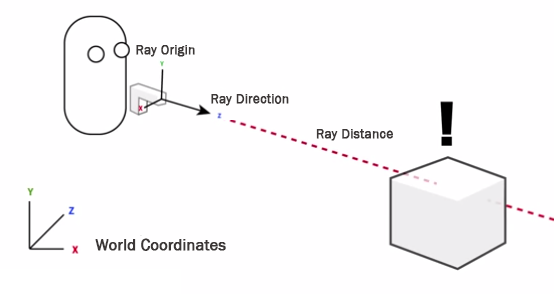
\includegraphics[width=0.8\textwidth]{Raycast}
    \caption{Funktionsweise des \textit{Raycastings}}
    \label{fig:Raycasting}
\end{figure}

Das ARKit-Framework bietet eine Funktion, mit der Raycasts innerhalb der AR-Szene durchgeführt werden können. Der Startpunkt und die Richtung des Strahls lassen sich über ein \texttt{RaycastQuery}-Objekt definieren. Die Funktion gibt ein Array von \texttt{ARRaycastResult}-Objekten zurück, die Informationen zu den Schnittpunkten des Strahls mit den getroffenen Objekten, deren Art und Orientierung enthalten. Falls das getroffene Objekt einen \texttt{ARAnchor} besitzt, wird auch dieser zurückgegeben.

Im Rahmen der Anwendung wurde Raycasting genutzt, um den Mindestabstand zu umliegenden Wänden zu validieren. Hierfür werden mehrere Raycasts parallel zur x-z-Ebene in einem 360-Grad-Winkel um die Focus-Entity geschossen, um die Umgebung auf zu nahe Wände zu überprüfen. Wenn ein Strahl auf ein Objekt trifft, wird davon ausgegangen, dass es sich um eine Wand oder ein Wand-ähnliches Objekt handelt. Anschließend wird der Abstand zwischen diesem Objekt und der Focus-Entity berechnet und mit dem festgelegten Mindestabstand verglichen. Liegt der Abstand unter dem definierten Wert, wird die Position der Focus-Entity als ungültig betrachtet und die Platzierung des virtuellen Rauchmelders verhindert.

[Bild: 360-Grad-Raycasting]

Darüber hinaus bildet Raycasting die Grundlage für die Positionierung der Focus-Entity. Bei jedem Frame wird ein Raycast von der Kamera in das Zentrum der AR-Szene abgefeuert, und die Position des ersten getroffenen Objekts wird als Position der Focus-Entity verwendet. Dies ermöglicht eine präzise Platzierung der Focus-Entity und eine genaue Ausrichtung des virtuellen Rauchmelders.

\subsection{Virtuelle Objekte der AR-Szene}

Die Entitäten (\textit{Entities}) der Augmented-Reality-Szene stellen die Model-Objekte des Prototypen dar. Dabei handelt es sich um virtuelle Objekte, die in der augmentierten Umgebung platziert werden und dem Benutzer eine visuelle Rückmeldung geben. Wie in Abbildung \ref{fig:Architecture} dargestellt, beschränken sich die visualisierten Entitäten auf die folgenden Objekte:

\begin{itemize}
    \item \texttt{FocusEntity}
    \item \texttt{SmokeDetector}
    \item \texttt{DistanceIndicators}
\end{itemize}

Diese Entitäten wurden so konzipiert, dass sie sich dynamisch an die Umgebung anpassen und direkt in der Augmented-Reality-Szene platziert werden können. Zur Umsetzung wurden Protokolle und Klassen des \texttt{RealityKit}-Frameworks genutzt. Im Beispiel der \texttt{SmokeDetector}-Entität wurde die Klasse wie folgt implementiert:

\begin{lstlisting}[language=Swift]
class SmokeDetector: Entity, HasModel, HasAnchoring {
    init() {
        super.init()
        // Initialization of MeshComponent and ModelComponent
    }
    // ...
}
\end{lstlisting}

Die Klasse \texttt{SmokeDetector} erbt von \texttt{Entity}, der grundlegenden Klasse für alle virtuellen Objekte in einer Augmented-Reality-Szene. Sie implementiert zudem das \texttt{HasModel}-Protokoll, das die Nutzung von 3D-Modellen innerhalb der Entität ermöglicht. Das \texttt{HasAnchoring}-Protokoll sorgt dafür, dass die Entität an einem AR-Anchor verankert werden kann. Änderungen an der Entität werden automatisch in der AR-Szene übernommen und visuell dargestellt.

Ein potenzieller Nachteil dieser Implementierung besteht darin, dass die \texttt{RealityKit}-Komponenten direkt in den Model-Klassen verwendet werden. Dies führt zu einer gewissen Abhängigkeit zwischen der Model- und der View-Schicht, wodurch die strikte Trennung der Architekturprinzipien – insbesondere des MVVM-Patterns – nicht vollständig eingehalten wird. Eine alternative Lösung wäre die vollständige Entkopplung der Model-Klassen von den AR-spezifischen Komponenten. Dies würde jedoch eine zusätzliche Abstraktionsebene und damit eine erhöhte Komplexität mit sich bringen.

Im Rahmen dieses Prototypen wurde daher ein pragmatischer Ansatz gewählt: Die direkte Integration der \texttt{RealityKit}-Komponenten innerhalb der Model-Klassen ermöglicht eine effizientere Entwicklung und eine schnellere Iteration, ohne die Wartbarkeit wesentlich zu beeinträchtigen.

\subsection{FocusEntity}

Die \texttt{FocusEntity} stellt die Grundlage der Interaktion des Benutzers mit der Augmented-Reality-Szene dar. Sie dient als visuelle Markierung, um den Benutzer bei der regelkonformen Platzierung des virtuellen Rauchmelders zu unterstützen. Die \texttt{FocusEntity} besteht aus zwei Komponenten: einer vereinfachten und einfarbigen Darstellung eines Rauchmelders und einem zweidimensionalen Ring. Der Ring visualisiert den Mindestabstand von 0,6 Metern zu umgebenden Wänden und wird nur angezeigt wenn die Decke als Zieloberfläche erkannt wurde. Zusätzlich dazu wird die Farbe der \texttt{FocusEntity} dynamisch angepasst, um dem Benutzer eine visuelle Rückmeldung über die Gültigkeit der aktuellen Position zu geben. Die Abbildung \ref{fig:AppUI} zeigt die \texttt{FocusEntity} in der Augmented-Reality-Szene.

Die Implementierung der \texttt{FocusEntity} orientiert sich an einer bereits existierenden Lösung \cite{cobb2019focusEntity}, wobei darauf geachtet wurde, die Entität in die Architektur des Prototypen zu integrieren und Abängigkeiten zu anderen Systemen zu minimieren. Im Folgenden werden die wichtigsten Aspekte der Implementierung erläutert.

Die Aktualisierung des Zustands der \texttt{FocusEntity} erfolgt über das \texttt{TrackingState}-Enum. Dieses Enum definiert zwei mögliche Zustände:

\begin{lstlisting}[language=Swift]
enum TrackingState: Equatable {
    case initializing
    case tracking(raycastResult: ARRaycastResult)
}
\end{lstlisting}

Abhängig von dem Ergebnis eines Raycasts, der in das Zentrum des Bildschirms geschossen wird, wird der Tracking-Zustand in einer \texttt{trackingState}-Variable gespeichert. Liefert der Raycast kein gültiges Ergebnis, wird der Zustand auf \texttt{initializing} gesetzt und die \texttt{FocusEntity} wird direkt vor der Kamera platziert. Andernfalls wird die \texttt{trackingState}-Variable mit dem Ergebnis des Raycasts aktualisiert und die Position der \texttt{FocusEntity} wird aktualisiert. Auf die Änderungen der \texttt{trackingState}-Variable wird mithilfe eines \textit{Property Observers} reagiert: 

\begin{lstlisting}[language=Swift]
var trackingState: TrackingState = .initializing {
    didSet {
        // ...
        switch trackingState {
        case .initializing:
            // Platziere die FocusEntity direkt vor der Kamera
        case .tracking(let raycastResult):
            // Aktualisiere die Position der FocusEntity
        }
    }
}
\end{lstlisting}

Die \texttt{didSet}-Methode wird aufgerufen, sobald sich der Wert der \texttt{trackingState}-Variable ändert. Abhängig vom neuen Zustand wird die Position der \texttt{FocusEntity} angepasst. Zur Stabilisierung der Position wird die neue Entitätsposition über die letzten zehn Frames hinweg gemittelt:

\begin{lstlisting}[language=Swift]
private func updatePosition() {
    recentFocusEntityPositions = Array(recentFocusEntityPositions.suffix(10))
    let average = recentFocusEntityPositions.reduce(
        SIMD3<Float>.zero, { $0 + $1 }
    ) / Float(recentFocusEntityPositions.count)
    self.position = average
    // ...
}
\end{lstlisting}

Zusätzlich wird überprüft, ob die Orientierung der \texttt{FocusEntity} aktualisiert werden soll. Dies erfolgt durch die Auswertung der letzten 20 \texttt{ARPlaneAnchor.Alignment}-Werte, die im \texttt{ARRaycastResult}-Objekt enthalten sind:

\begin{lstlisting}[language=Swift]
self.recentFocusEntityAlignments = Array(self.recentFocusEntityAlignments.suffix(20))
let alignCount = self.recentFocusEntityAlignments.count
let horizontalHistory = recentFocusEntityAlignments.filter({ $0 == .horizontal }).count
let verticalHistory = recentFocusEntityAlignments.filter({ $0 == .vertical }).count
if alignment == .horizontal && horizontalHistory > alignCount * 3/4 ||
    alignment == .vertical && verticalHistory > alignCount / 2 ||
    raycastResult.anchor is ARPlaneAnchor {
    // Aktualisiere die Orientierung der FocusEntity
}
\end{lstlisting}

Hierbei wird die Anzahl der horizontalen und vertikalen Ausrichtungen überprüft. Überschreitet eine dieser Ausrichtungen einen festgelegten Schwellenwert, wird die Orientierung der \texttt{FocusEntity} aktualisiert, sofern diese Ausrichtung nicht bereits die aktuelle ist.

Falls das \texttt{ARRaycastResult} keinen \texttt{ARPlaneAnchor} enthält und der Fokus daher nicht auf einer erkannten Fläche liegt, wird die \texttt{FocusEntity} auf die Orientierung des Zielpunkts des \texttt{ARRaycastResult} ausgerichtet. Dies ermöglicht eine präzise Platzierung der \texttt{FocusEntity} auf beliebigen Oberflächen, auch wenn diese nicht als erkannte Flächen identifiziert wurden.

\subsection{Performance-Optimierung}

Wie in den Anforderungen betont, ist die Performance ein entscheidender Faktor bei der Entwicklung von Augmented-Reality-Anwendungen. Sie wird von verschiedenen Aspekten beeinflusst, darunter die Verarbeitungsgeschwindigkeit der Sensordaten, die Darstellung virtueller Objekte und die Benutzerinteraktion. Um eine hohe Performance zu gewährleisten, wurden gezielte Optimierungsmaßnahmen implementiert, die sowohl die Datenverarbeitung effizienter gestalten als auch die Darstellung der AR-Szene beschleunigen.

Zunächst lag der Fokus auf der Verbesserung der synchronen Implementierung, bevor Multithreading als Optimierungsstrategie in Betracht gezogen wurde. Drei wesentliche Maßnahmen wurden identifiziert, um die Performance zu steigern:

\begin{itemize}
\item Reduktion der Verarbeitungsfrequenz der ARFrame-Daten
\item Optimierung der Raycast-Abstandsprüfung
\item Filterung der ARMeshAnchors zur effizienteren Abstandsanalyse
\end{itemize}

Die Verarbeitung der ARFrame-Daten wurde optimiert, indem die Regelprüfung nur noch alle zehn Frames ausgeführt wird. Diese Reduktion der Berechnungsfrequenz verringert die Anzahl der Operationen erheblich.

Die Anzal der Raycasts zur Abstandskontrolle wurde zunächst auf 30 gesetzt, um die nicht abgedeckten Winkelbereiche zu minimieren. Tests haben jedoch gezeigt, dass eine geringere Anzahl von Raycasts ausreicht, um die notwendigen Informationen zu erhalten. Aus diesem Grund wurde die Anzahl der Raycasts auf 9 reduziert, was zu einer deutlichen Effizienzsteigerung bei der Überprüfung der Abstände führt.

Darüber hinaus wurde die Analyse der ARMeshAnchors optimiert, indem eine Vorabfilterung durchgeführt wird: Anker, die sich außerhalb des festgelegten Mindestabstands zu Türen und Fenstern befinden, werden bereits im Vorfeld ausgeschlossen. Dies reduziert die Anzahl der zu überprüfenden Anker erheblich und beschleunigt die Abstandskontrollen.

Dank dieser Maßnahmen konnte die Performance der Anwendung deutlich verbessert werden, ohne dass sofort auf parallele Verarbeitung zurückgegriffen werden musste.

Im nächsten Schritt wurde Multithreading eingeführt, um die Verarbeitung der ARFrame-Daten weiter zu beschleunigen. Dabei wurde das \texttt{async/await}-Feature von Swift genutzt, das eine einfache und effiziente Handhabung asynchroner Operationen ermöglicht. Die Funktionen zur Überprüfung der Montageregeln wurden in einen separaten Thread ausgelagert, wodurch die Hauptverarbeitungsschleife und damit die \texttt{ARView} nicht blockiert wird. Diese Maßnahme verbessert die Reaktionszeit der Anwendung und steigert die Gesamtperformance.